\documentclass[10pt,a4paper]{article}
\usepackage[utf8]{inputenc}
\usepackage{amsmath}
\usepackage{amsfonts}
\usepackage{amssymb}
\usepackage{graphicx}
\usepackage{enumerate}
\begin{document}

\section{Set Theory}

To demystify mathematics consider
\begin{enumerate}[(i)]
\item What is a theorem?
\item What is a proof?
\end{enumerate}
What if we don't know the answer?

To begin we need
\begin{enumerate}[(a)]
\item an example(s)
\item a nearly related concept
\end{enumerate}


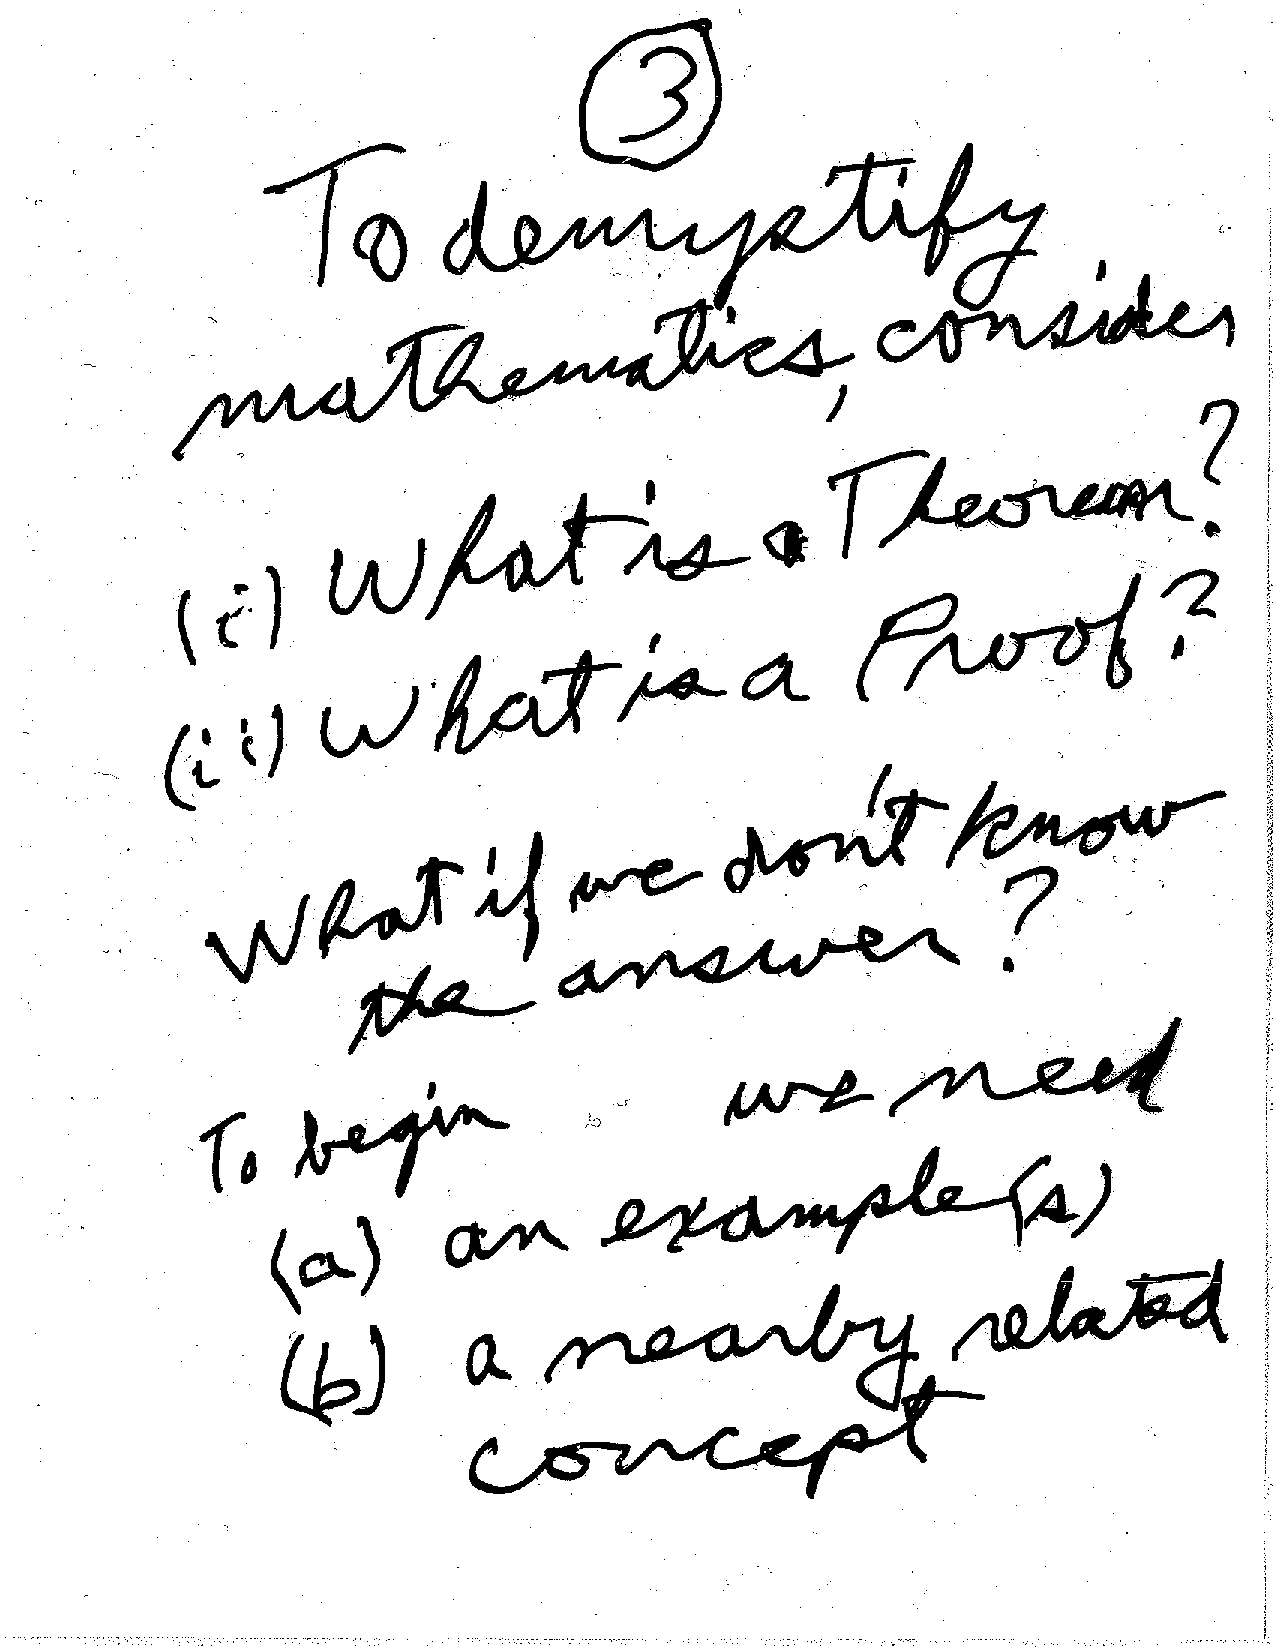
\includegraphics[scale=.5]{Pages/ST_3}

\newpage

Related Concept: Greek Syllogism

\underline{example:}
\begin{enumerate}
\item All men are mortal.
\item Socrates is a man.
\item Therefore, Socrates must die. 
\end{enumerate}

To analyze, recast in set theoretic terms via Venn Diagram.

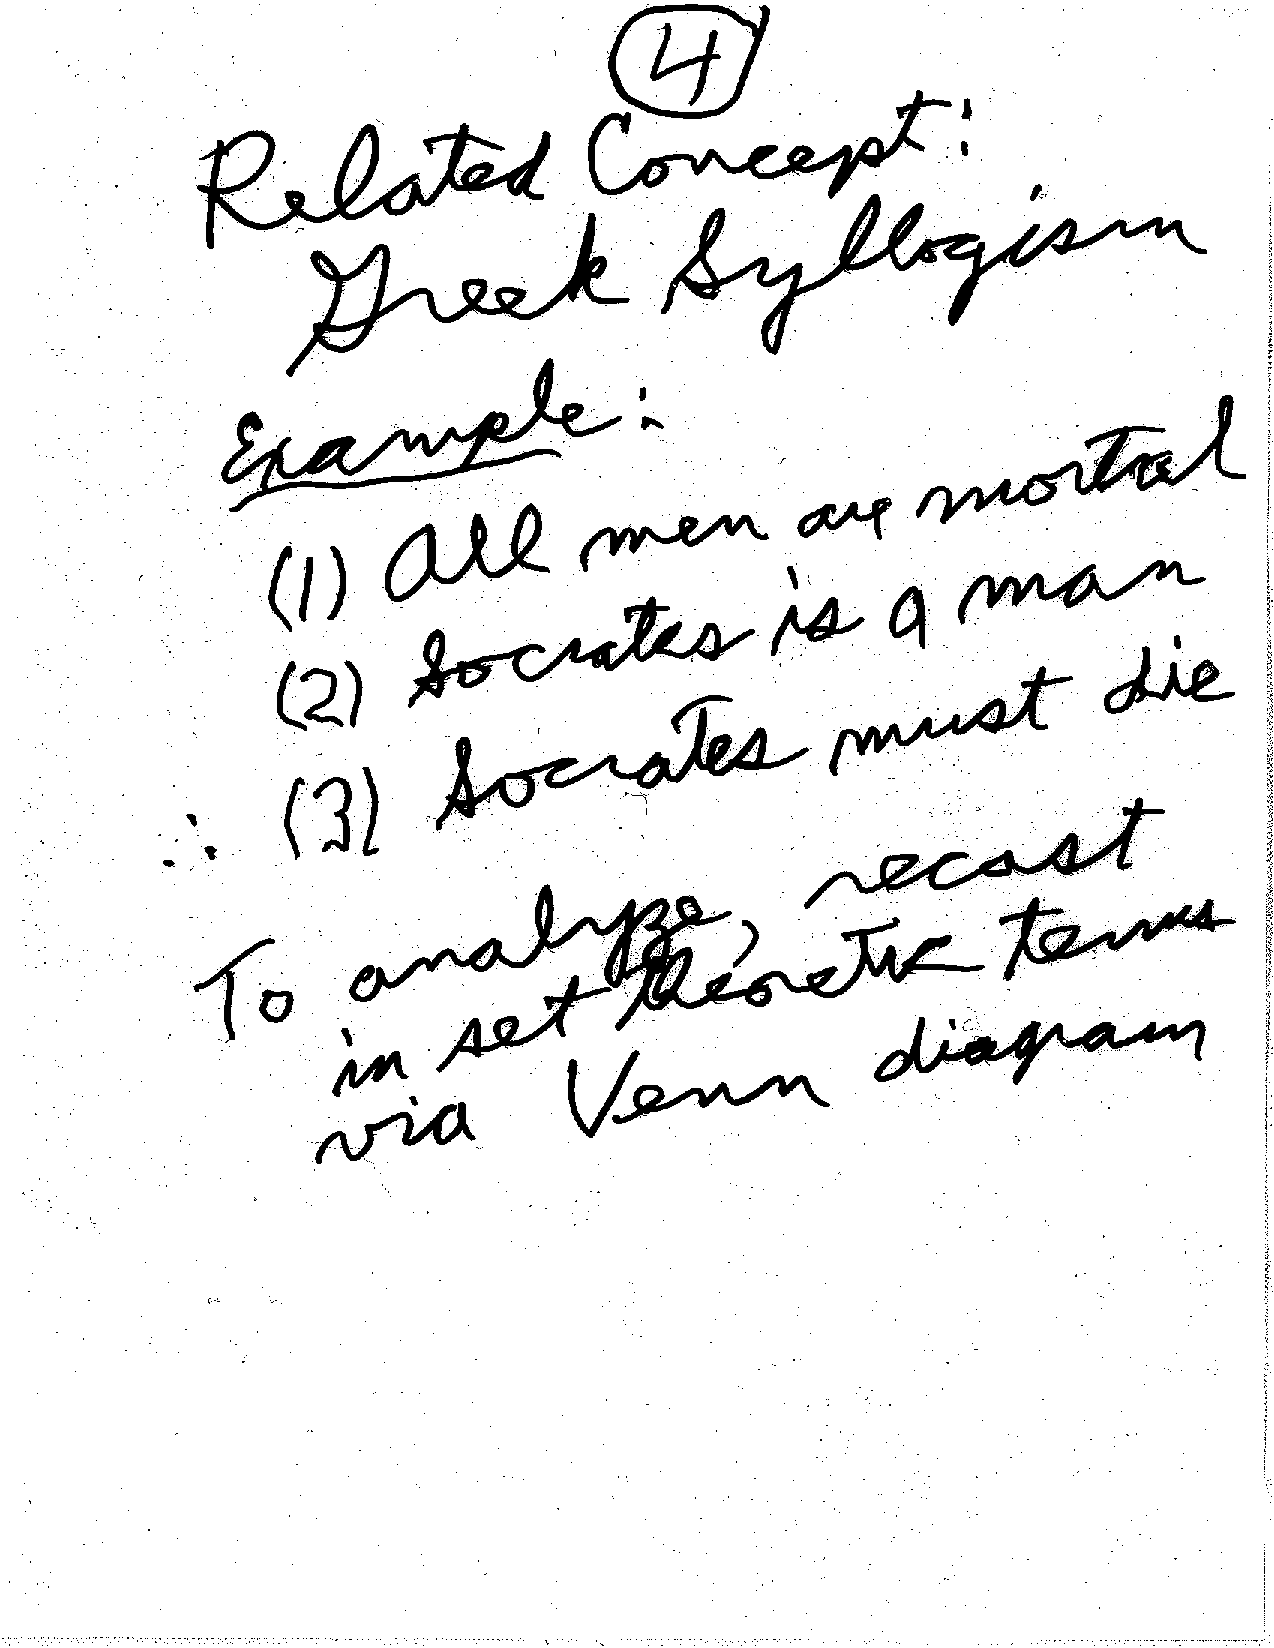
\includegraphics[scale=.5]{Pages/ST_4}

\newpage

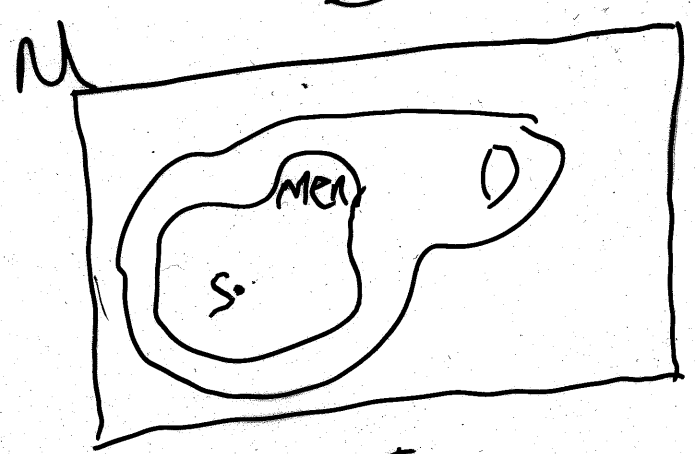
\includegraphics[scale=.2]{Pages/ST_5_im1}

$S$: Socrates\\
$M$: Set of Men\\
$D$: Things that will die\\
$\mathcal{U}$: Things on Earth

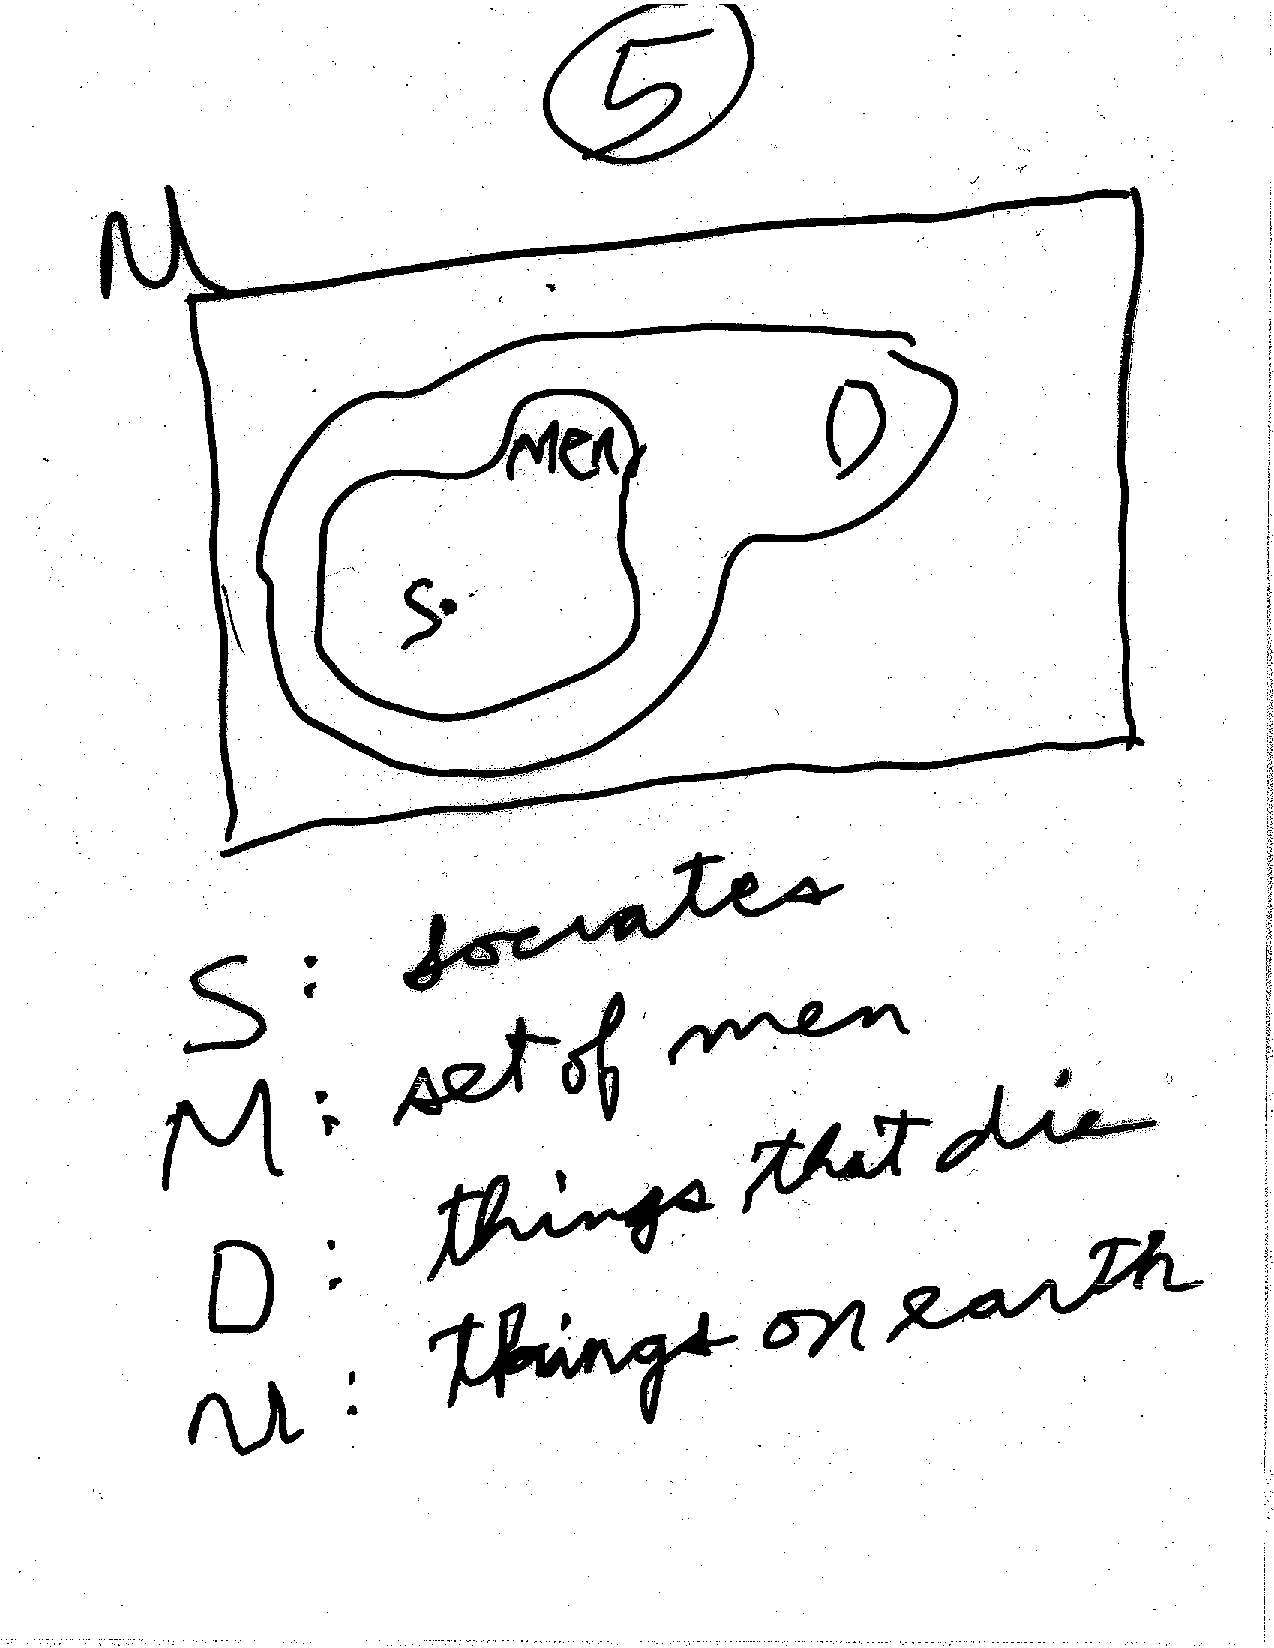
\includegraphics[scale=.5]{Pages/ST_5} 



%Zack: Pages 6,7,8,19,20

%Jack: 21, 9, 10, 11

%Koka: Pages 13, 13A, 22 ,22A, 22B


\section{Generate $\mathbb{N}$}


%Ruth: Pages L4A-L4G




\section{From $\mathbb{Z}$ to $\mathbb{R}$ via ordering}
%Jazz: ZR1-ZR5

%Kyler: ZR6 - ZR10

ZR6

 
Continuing in this way we generate 

$(\mathbb{Z}_{2^k},<2_{2^k})$ For all $k\in\mathbb{N}$
                     


Then we get 

\quad\quad\quad$\infty$
           
$\mathbb{Z}_{\infty} = \bigcup$ $Z_{(2k)}$ 

  \quad\quad $k=1$

Problem: How do we put an ordering $<_{\infty}$ on $Z_{(\infty)}$ 

That extends every $<_{2k}$?

\quad
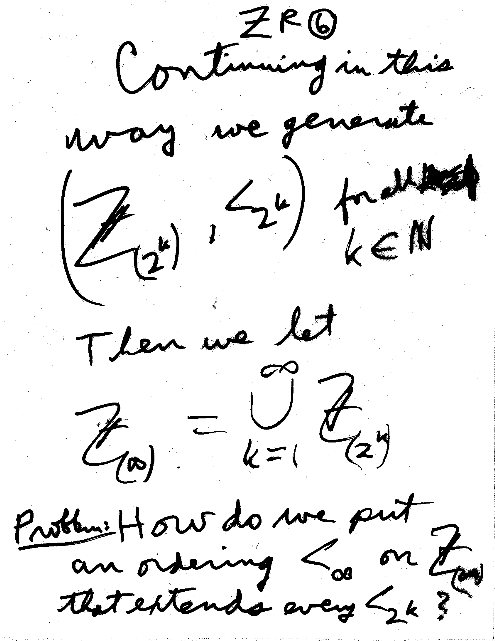
\includegraphics[scale=0.6]{Pages/ZR6.png}

\newpage 
\title{ZR7}
\maketitle

We can represent $\mathbb{Z}$ in terms of integers $j,k,n$ and that $\mathbb{Z} _{\infty} = \mathbb{Z}\bigcup$ $\left\{n+\frac{j}{2k} = k\geqslant1 and \lneqq j < z^k\right\}$

What does the ordering look like? 

Suppose we want to construct a version of $\mathbb{Z}_{(\infty)}$ that exhibits.  

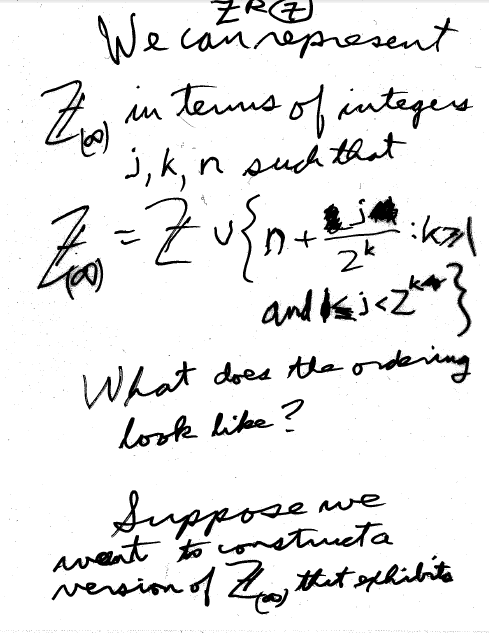
\includegraphics[scale=0.6]{Pages/ZR7.png} 

\newpage 

\title{ZR8}

\maketitle 

The ordering. 
for $x\in \mathbb{Z}_{\infty}$ let 

$L_{x}=\left\{y\in\mathbb{Z}:y<_{\infty}x\right\}$

Now $L_{x}$ denotes the dyadic rational x. 

notice that for any 

$x,y$ in $\mathbb{Z}_{\infty},$ 

$L_{x} \bigcup L_{y} = L_{w}$ for 

$w=x$ or $w=0$ 

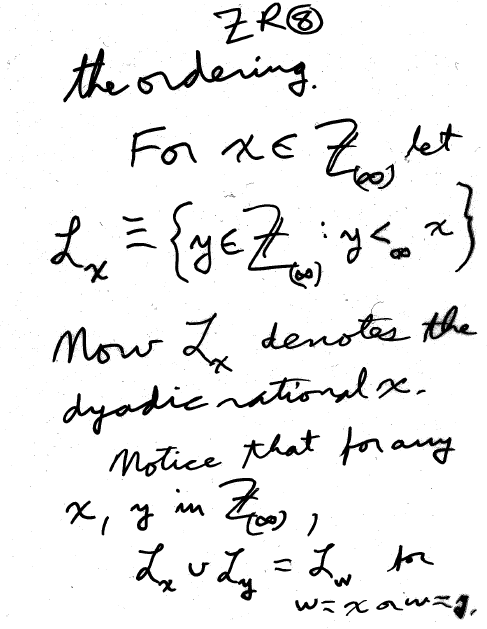
\includegraphics[scale=0.6]{pages/ZR8.png}

\newpage

\title{ZR9} 

\maketitle

Hence for any $n\geqslant1$ and $x,..., x_{n} \in \mathbb{Z}_{\infty}$
  


    $\bigcup_{j=1}^{n} L_{x_j} = L_{w}$ 
   
                          
               
      
       For w $\in$ $\bigcup_{j=1}^{n}$ $\left\{x_{j}\right\}$
                         
                          
               
Hence, finite unions of dyadic rationals one dyadic rationals suppose we want to think of arbitrary unions of 
$L{x}= x\in\mathbb{Z}_{\infty}$ as bone fide numbers. 

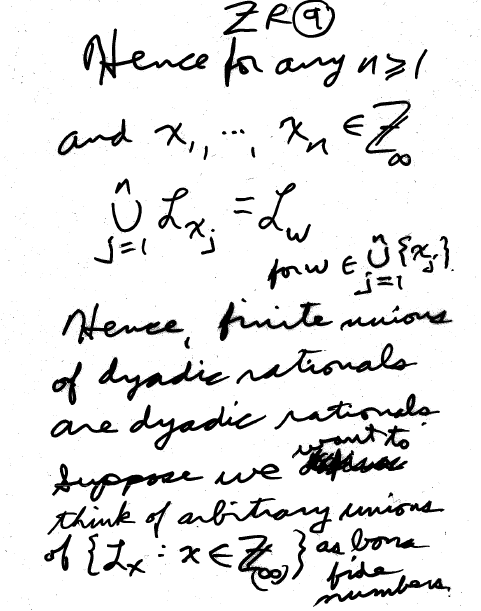
\includegraphics[scale=0.6]{pages/ZR9.png}

\newpage

ZR10



LET 

$R_{\infty}$ = $\left\{\bigcup_{X\in A} L_{x} = a\subseteq\mathbb{Z}_{\infty}\right\}$
         
            

Letting $A=\emptyset, \emptyset\in R_{\infty}$ 

Letting $A=\mathbb{N}, \mathbb{Z}_{\infty}\in R_{\infty}$

Let $R=\left\{B\in R_{\infty}:B\neq\emptyset \mbox{ and } B\neq\mathbb{Z}_{(\infty)}\right\}$  

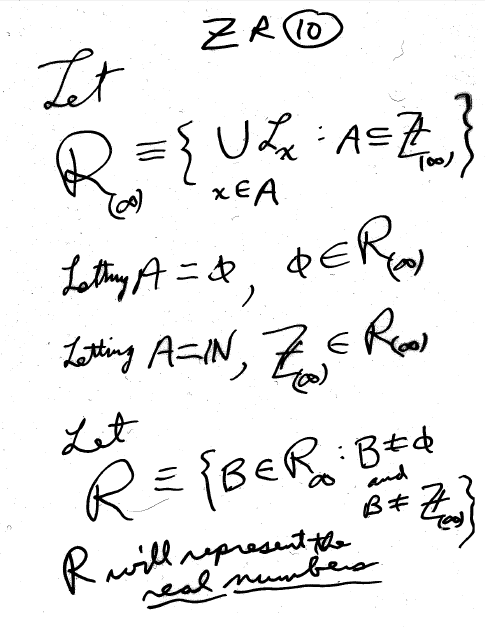
\includegraphics[scale=0.6]{pages/ZR10.png}

R will represent real numbers 
%Preethika: ZR11-ZR14


\section{Sequence and Limits}

%Aaron: First 2 pages and 48-50

%Hamza: 51-52B

\section{Limit and Convergence}

%Joe: 50-51

%Quinten: 52-53

%Farishta: 53A-54A

\section{Infinite Series}

%Sukhreet: IS1 - IS 7

%Matthew: IS8 - IS15

%Will: IS16 - IS23

%Rebecca: IS24 - IS32

%Maady: IS33 - IS42

\section{Metric Spaces Part 1}

%Travis: M1 - M5

%Jerome: M6- M10



\section{Metric Spaces Part 2}


%Bryant: M1-M7

%Reshma: M8-M14

%Ethan: M15-M21





\end{document}